\documentclass[../main.tex]{subfiles}
\begin{document}
\section{Protocolos}

Hasta ahora teníamos primitivas sueltas: confidencialidad (cifrado), integridad
(MAC/hash), cifrado autenticado, criptografía asimétrica y firma digital. Esta
unidad las \textbf{compone} en \emph{protocolos}: secuencias de mensajes que, sobre
un canal inseguro, le dan a las partes confidencialidad, integridad y autenticación
de quién está del otro lado. Cierra con un tema aparte —el \textbf{secreto
compartido de Shamir}— que se toma mucho en el segundo parcial.

\prof{Ahora lo que estamos haciendo es componer las piezas para poder hacer lo que queremos, que es transmitir información de forma que llegue solo a quien queremos, con garantía de que no fue alterada y de que somos verdaderamente la entidad que la emitió.}

\subsection{Qué es un protocolo criptográfico}

Un criptosistema CCA-Secure permite enviar $\mathrm{Enc}_k(M)$ manteniendo
\textbf{confidencialidad} e \textbf{integridad}, \emph{pero requiere que ambas
partes conozcan una misma clave $k$}. El problema central de los protocolos es
justamente cómo llegar a esa clave compartida y cómo garantizar con quién se habla.

\paragraph{Protocolo de intercambio de claves.} Es un protocolo $\Pi(n)$ ejecutado
por dos partes:
\begin{itemize}[leftmargin=1.4em]
  \item $\Pi: (n) \to \mathrm{Tran},\, k_a,\, k_b$.
  \item \textbf{No tiene entrada}, salvo el parámetro de seguridad $n$ (que fija la
  longitud de las claves, es decir la seguridad computacional).
  \item La salida es: un conjunto de mensajes intercambiados (la \emph{traza} o
  \emph{log}), una clave $k_a$ conocida solo por una de las partes y una clave $k_b$
  conocida solo por la otra.
  \item \textbf{Condición fundamental de correctitud:} $k_a = k_b$ (ambos llegan a
  la misma clave).
\end{itemize}

\paragraph{Tipos de ataque que se quieren evitar.}
\begin{itemize}[leftmargin=1.4em]
  \item \textbf{Ataques pasivos (snooping):} el atacante solo mira los mensajes e
  intenta deducir la clave o los datos.
  \item \textbf{Ataques activos:} el atacante juega un rol dentro del protocolo.
  Puede \emph{omitir} mensajes, \emph{reescribir} su contenido, \emph{reordenarlos}
  o \emph{repetirlos}. Aparece el \textbf{Man-in-the-Middle (MitM)}: el atacante se
  para en el medio y le hace creer a cada lado que es la contraparte.
\end{itemize}

\begin{definicion}{Nonce y frescura}
Un \textbf{nonce} (number used once) es un número aleatorio de un solo uso. Aporta
\textbf{frescura}: permite atar un mensaje a una ejecución concreta del protocolo y
así detectar/evitar \textbf{replays} (repeticiones de mensajes viejos). El otro
mecanismo de frescura es el \textbf{timestamp} (marca de tiempo).
\end{definicion}

\subsection{Distribución de claves: KDC (simétrico) vs PKI (asimétrico)}

El problema de la clave simétrica es \emph{cómo distribuirla}. Hay dos grandes
enfoques.

\paragraph{Esquema simétrico: KDC.} Existe un tercero de confianza, el
\textbf{KDC} (Key Distribution Center). \emph{Hipótesis de arranque:} cada entidad
\textbf{ya comparte una clave con el KDC} (se estableció físicamente / fuera de
banda). El KDC genera claves de sesión entre pares. Es la base de \textbf{Kerberos}
y de Active Directory (con modificaciones).

\paragraph{PGP (mencionado).} Protocolo antiguo (Pretty Good Privacy, años '90)
basado en \emph{delegación / transferencia de confianza}: yo confío en alguien que
vi físicamente, y le sirvo de ``KDC'' a un tercero, encadenando confianza (incluso
con grados). Ya no se ve en la materia porque casi no se usa.

\paragraph{Esquema asimétrico: PKI.} En el mundo de clave pública el equivalente del
KDC es la \textbf{PKI} (Public Key Infrastructure). Resuelve el problema de asociar
una \textbf{clave pública} con una \textbf{identidad}. El ataque que busca evitar es
el MitM/\emph{spoofing}: si $A$ pide ``la clave de $B$'' y un atacante $E$ le
responde con $pk_e$ en vez de $pk_b$, $A$ cree hablar con $B$ pero en realidad cifra
con la clave de $E$. \textbf{No es aplicable a criptosistemas simétricos.}

\begin{examen}
\textbf{KDC vs PKI (2016, 2018, 2023).} Hay que poder explicar similitudes y
diferencias:
\begin{itemize}[leftmargin=1.3em]
  \item \textbf{Similitud:} ambos descansan en un \textbf{tercero de confianza} y un
  punto de anclaje (la clave compartida con el KDC; los certificados raíz en PKI).
  \item \textbf{KDC:} simétrico, \emph{online} (el KDC participa activamente en cada
  intercambio), conoce/maneja las claves. Si el KDC se compromete, todo deja de
  tener sentido.
  \item \textbf{PKI:} asimétrico, las CA firman certificados que pueden validarse
  \emph{offline}; la CA no necesita estar online en cada comunicación. La confianza
  forma un árbol/cadena hasta una raíz autofirmada.
\end{itemize}
\end{examen}

\subsubsection{Análisis de protocolos KDC: Needham-Schroeder paso a paso}

Notación: $\{M\}_k = e_k(M)$ (todo lo que está entre llaves está cifrado con $k$).
$k_a$ = clave de $A$ con el KDC, $k_b$ = clave de $B$ con el KDC, $k_s$ = clave de
sesión nueva.

\paragraph{Primera aproximación (insegura).}
\begin{align*}
A &\to \text{KDC}: \quad \{\text{Sesión } A \to B\}_{k_a} \\
\text{KDC} &\to A: \quad \{k_s\}_{k_a} \,\|\, \{k_s\}_{k_b} \\
A &\to B: \quad \{k_s\}_{k_b}
\end{align*}
\textbf{Problemas:}
\begin{itemize}[leftmargin=1.4em]
  \item \textbf{Replay:} un atacante graba $\{k_s\}_{k_b}$ y lo reenvía; $B$ no tiene
  forma de saber que no está hablando con $A$.
  \item \textbf{Key reuse:} un atacante graba el mensaje del KDC y se lo reenvía a
  $A$ cuando $A$ inicia otra conversación; $A$ y $B$ terminan usando la misma clave
  de sesión vieja.
\end{itemize}

\paragraph{Segunda aproximación (con nonces).}
\begin{align*}
A &\to \text{KDC}: \quad A \to B \,\|\, r_1 \\
\text{KDC} &\to A: \quad \{\, A \,\|\, B \,\|\, r_1 \,\|\, k_s \,\|\, \{A \,\|\, k_s\}_{k_b}\,\}_{k_a} \\
A &\to B: \quad \{A \,\|\, k_s\}_{k_b} \\
B &\to A: \quad \{r_2\}_{k_s} \\
A &\to B: \quad \{r_2 - 1\}_{k_s}
\end{align*}

\begin{center}
\begin{tikzpicture}[font=\small,
  msg/.style={-{Stealth}, thick},
  lbl/.style={midway, above, font=\scriptsize}]
  % lifelines: A, KDC, B
  \def\ax{0} \def\tx{5.6} \def\bx{11}
  \def\ytop{0.4} \def\ybot{-7.2}
  % heads
  \node[draw, fill=blue!8, minimum width=1.1cm] (A) at (\ax,\ytop) {$A$};
  \node[draw, fill=orange!12, minimum width=1.3cm] (T) at (\tx,\ytop) {KDC};
  \node[draw, fill=green!10, minimum width=1.1cm] (B) at (\bx,\ytop) {$B$};
  % lifelines
  \draw[dashed, gray] (\ax,\ytop-0.3) -- (\ax,\ybot);
  \draw[dashed, gray] (\tx,\ytop-0.3) -- (\tx,\ybot);
  \draw[dashed, gray] (\bx,\ytop-0.3) -- (\bx,\ybot);
  % messages
  \draw[msg] (\ax,-0.7) -- (\tx,-0.7) node[lbl]{(1)\ $A \to B \,\|\, \mathbf{r_1}$};
  \draw[msg] (\tx,-2.0) -- (\ax,-2.0) node[lbl]{(2)\ $\{A \,\|\, B \,\|\, \mathbf{r_1} \,\|\, k_s \,\|\, \{A \,\|\, k_s\}_{k_b}\}_{k_a}$};
  \draw[msg] (\ax,-3.6) -- (\bx,-3.6) node[lbl]{(3)\ $\{A \,\|\, k_s\}_{k_b}$\quad(ticket)};
  \draw[msg] (\bx,-5.0) -- (\ax,-5.0) node[lbl]{(4)\ $\{\mathbf{r_2}\}_{k_s}$\quad(desafío de $B$)};
  \draw[msg] (\ax,-6.4) -- (\bx,-6.4) node[lbl]{(5)\ $\{\mathbf{r_2}-1\}_{k_s}$\quad(respuesta de $A$)};
  % nonce annotations
  \node[red, font=\scriptsize, anchor=west] at (\ax+0.1,-1.35) {$\mathbf{r_1}$: frescura $A\to$KDC};
  \node[red, font=\scriptsize, anchor=east] at (\bx-0.1,-5.7) {$\mathbf{r_2}$: frescura $B\to A$};
\end{tikzpicture}
\end{center}
\diagcaption{Needham--Schroeder (2.\textsuperscript{a} aproximación). El KDC ($T$) genera la clave de sesión $k_s$; los nonces $r_1$ (rojo, mensajes 1--2) y $r_2$ (rojo, mensajes 4--5) aportan frescura y evitan replays. El mensaje (3) es el \emph{ticket} cifrado con $k_b$ que solo $B$ puede abrir.}

\textbf{Por qué funciona:}
\begin{itemize}[leftmargin=1.4em]
  \item \textbf{2.º mensaje:} cifrado con $k_a$ (compartida $A$--KDC) $\Rightarrow$
  proviene del KDC; trae el $r_1$ que $A$ envió $\Rightarrow$ no es replay (frescura).
  \item \textbf{4.º mensaje:} solo $B$ puede enviarlo (sabe $k_s$); avisa a $A$ un
  intento de comunicación con un nonce fresco $r_2$.
  \item \textbf{5.º mensaje:} $A$ confirma; $B$ sabe que no es repetición porque
  recibe $r_2 - 1$ (demuestra que $A$ ``está vivo'' y leyó $r_2$).
\end{itemize}

\begin{ojo}
\textbf{El nombre del destinatario importa.} Incluir $B$ dentro del bloque cifrado
por el KDC evita que ese ticket se reuse para hablar con otra entidad: ata la clave
de sesión a un par concreto $A$--$B$.
\end{ojo}

\paragraph{El problema que queda (replay de clave de sesión vieja comprometida).}
Si el atacante $E$ consigue una \textbf{clave de sesión antigua} $k_s$, arranca
directo por el \textbf{tercer paso}:
\begin{align*}
E &\to B: \quad \{A \,\|\, k_s\}_{k_b} \quad \text{(mensaje viejo grabado)}\\
B &\to E: \quad \{r_2\}_{k_s} \\
E &\to B: \quad \{r_2 - 1\}_{k_s}
\end{align*}
Como $E$ conoce $k_s$, completa el challenge y \textbf{logra impersonar a $A$}. La
causa: \emph{$B$ no estuvo involucrado desde el principio}, no tiene cómo verificar
frescura del ticket.

\paragraph{Modificación Denning-Sacco: timestamps.} El arreglo propuesto es agregar
un \textbf{timestamp $T$} dentro del bloque destinado a $B$:
\begin{align*}
A &\to \text{KDC}: \quad A \,\|\, B \,\|\, r_1 \\
\text{KDC} &\to A: \quad \{\, A \,\|\, B \,\|\, r_1 \,\|\, k_s \,\|\, \{A \,\|\, T \,\|\, k_s\}_{k_b}\,\}_{k_a} \\
A &\to B: \quad \{A \,\|\, T \,\|\, k_s\}_{k_b} \\
B &\to A: \quad \{r_2\}_{k_s} \\
A &\to B: \quad \{r_2 - 1\}_{k_s}
\end{align*}
Ahora $B$ chequea que $T$ no sea viejo $\Rightarrow$ no se puede reutilizar un ticket
antiguo (rompe el replay/key-reuse). Esta variante con timestamp es la idea de
\textbf{Kerberos}.

\begin{center}
\begin{tikzpicture}[font=\small,
  msg/.style={-{Stealth}, thick},
  lbl/.style={midway, above, font=\scriptsize}]
  \def\ax{0} \def\tx{5.6} \def\bx{11}
  \def\ytop{0.4} \def\ybot{-7.2}
  \node[draw, fill=blue!8, minimum width=1.1cm] (A) at (\ax,\ytop) {$A$};
  \node[draw, fill=orange!12, minimum width=1.3cm] (T) at (\tx,\ytop) {KDC};
  \node[draw, fill=green!10, minimum width=1.1cm] (B) at (\bx,\ytop) {$B$};
  \draw[dashed, gray] (\ax,\ytop-0.3) -- (\ax,\ybot);
  \draw[dashed, gray] (\tx,\ytop-0.3) -- (\tx,\ybot);
  \draw[dashed, gray] (\bx,\ytop-0.3) -- (\bx,\ybot);
  \draw[msg] (\ax,-0.7) -- (\tx,-0.7) node[lbl]{(1)\ $A \,\|\, B \,\|\, r_1$};
  \draw[msg] (\tx,-2.0) -- (\ax,-2.0) node[lbl]{(2)\ $\{A \,\|\, B \,\|\, r_1 \,\|\, k_s \,\|\, \{A \,\|\, \mathbf{T} \,\|\, k_s\}_{k_b}\}_{k_a}$};
  \draw[msg] (\ax,-3.6) -- (\bx,-3.6) node[lbl]{(3)\ $\{A \,\|\, \mathbf{T} \,\|\, k_s\}_{k_b}$};
  \draw[msg] (\bx,-5.0) -- (\ax,-5.0) node[lbl]{(4)\ $\{r_2\}_{k_s}$};
  \draw[msg] (\ax,-6.4) -- (\bx,-6.4) node[lbl]{(5)\ $\{r_2-1\}_{k_s}$};
  \node[red, font=\scriptsize, anchor=west] at (\bx-3.0,-4.25) {$B$ verifica $\mathbf{T}$ fresco};
\end{tikzpicture}
\end{center}
\diagcaption{Variante Denning--Sacco: se agrega un \textbf{timestamp $T$} (rojo) dentro del ticket destinado a $B$ en los mensajes (2) y (3). Al recibir (3), $B$ comprueba que $T$ no sea viejo, lo que impide reutilizar un ticket/clave de sesión antiguo. Es la idea base de Kerberos.}

\begin{examen}
\textbf{Ejercicio estrella: ``analizar un protocolo'' (Ej.1 reciente).} Método para
los handshakes tipo Needham-Schroeder (2018):
\begin{enumerate}[leftmargin=1.5em]
  \item \textbf{Identificar el tipo:} intercambio de claves con KDC / tercero $T$.
  \item Para cada mensaje preguntarse \emph{quién lo pudo generar} (qué clave lo
  cifra) y \emph{qué garantiza} (frescura por nonce/timestamp, identidad por el
  nombre incluido, anti-replay).
  \item \textbf{Detectar el ataque:} típicamente \emph{replay de una clave de sesión
  vieja comprometida} porque el destinatario no participó desde el inicio.
  \item \textbf{Proponer el arreglo:} Denning-Sacco agrega \textbf{timestamps} para
  frescura/anti-replay (o atar la comunicación con $B$ desde el primer mensaje).
\end{enumerate}
\end{examen}

\begin{examen}
\textbf{Ataque por reflexión (2015).} En un protocolo de challenge-response con
nonces (firma del desafío), $C$ se autentica como $A$ \textbf{abriendo una sesión
paralela} y reusando el desafío que recibió: le pide a $A$ que le firme/responda su
propio challenge y lo refleja en la sesión original. \emph{Defensa:} romper la
simetría de los mensajes (incluir identidades/dirección, nonces distintos por
sentido).

\begin{center}
\begin{tikzpicture}[font=\small,
  msg/.style={-{Stealth}, thick},
  lbl/.style={midway, above, font=\scriptsize}]
  \def\ax{0} \def\cx{11}
  \def\ytop{0.4} \def\ybot{-6.6}
  \node[draw, fill=blue!8, minimum width=1.1cm] (A) at (\ax,\ytop) {$A$};
  \node[draw, fill=red!12, minimum width=1.1cm] (C) at (\cx,\ytop) {$C$ (impostor)};
  \draw[dashed, gray] (\ax,\ytop-0.3) -- (\ax,\ybot);
  \draw[dashed, gray] (\cx,\ytop-0.3) -- (\cx,\ybot);
  % session 1 (original): C se hace pasar por A frente a A
  \draw[msg] (\cx,-0.7) -- (\ax,-0.7) node[lbl]{Sesión 1: $C$ inicia, $A$ manda desafío $\mathbf{r}$};
  % A responds with r as challenge -- C cannot answer
  \draw[msg, dashed] (\cx,-1.7) -- (\ax,-1.7) node[lbl, text=red]{$C$ no sabe responder $f(\mathbf{r})$\dots};
  % session 2 parallel: C opens new session and reflects r
  \draw[msg] (\cx,-3.1) -- (\ax,-3.1) node[lbl]{Sesión 2 (paralela): $C$ reenvía el mismo desafío $\mathbf{r}$};
  \draw[msg] (\ax,-4.1) -- (\cx,-4.1) node[lbl]{$A$ responde $f(\mathbf{r})$ (firma su propio desafío)};
  % C reflects answer back into session 1
  \draw[msg] (\cx,-5.5) -- (\ax,-5.5) node[lbl, text=red]{Sesión 1: $C$ refleja $f(\mathbf{r})$ $\Rightarrow$ se autentica como ``$A$''};
\end{tikzpicture}
\end{center}
\diagcaption{Ataque por reflexión. $C$ no puede responder el desafío $r$ que le pide $A$; abre una \textbf{sesión paralela} (sesión 2), le reenvía el mismo $r$ a $A$ y obtiene $f(r)$, que luego \emph{refleja} en la sesión original. Defensa: romper la simetría (incluir identidad/dirección, nonces distintos por sentido).}
\end{examen}

\subsection{Certificados y PKI}

\begin{definicion}{Certificado}
Mensaje que asocia una \textbf{clave pública} a una \textbf{identidad}. Contiene al
menos: información de identidad (ej.\ nombre), la clave pública asociada, fecha de
emisión, intervalo de validez y \textbf{tipo de uso} de la clave (firma de mensajes,
cifrado de emails, firma de certificados, cifrado de sitios web). Está
\textbf{firmado digitalmente por una autoridad competente (CA)}.
\end{definicion}

\paragraph{Cómo se autoprotege el certificado (integridad intrínseca).} Se toma toda
la información del certificado (incluida la clave pública del sujeto), se le calcula
un \textbf{hash} y ese hash se firma con la \textbf{clave privada de la CA}; la firma
se adosa al certificado. Si se altera \emph{cualquier} bit (incluidos los bits de la
firma), la firma deja de validar $\Rightarrow$ se detecta. Por eso el certificado
puede distribuirse públicamente (lo puede dar el propio $B$).

\prof{La clave pública se distribuye firmada con la clave privada de la autoridad certificante.}

\paragraph{Uso del certificado por $A$.} $A$ solicita el certificado de $B$ (puede
darlo $B$ o cualquiera) y puede:
\begin{itemize}[leftmargin=1.4em]
  \item \textbf{Verificar la identidad:} comparar el \textbf{CN} (Common Name) con lo
  que espera. Ej.: para sitios web, CN = dominio (\texttt{mipanaderia.com}); para
  email, CN = dirección; para servidores, CN = IP/hostname; para empresas, CN = razón
  social. El browser, al conectarse a \texttt{santander.com}, exige que el CN
  coincida con el hostname al que se conecta; si no, corta.
  \item \textbf{Obtener la clave pública} de $B$ (está en el propio certificado,
  junto con el tipo: RSA-2048, DSA-EC 320, etc.).
  \item \textbf{Verificar validez:} tipo de uso permitido y fecha de vigencia.
  \item \textbf{Verificar integridad:} validar la firma digital de la CA (requiere la
  clave pública de la CA).
\end{itemize}

\subsubsection{Cadenas de firmas y CA raíz}

Las CA tienen a su vez un certificado, firmado por otra CA, y así hasta llegar a las
\textbf{CA raíz}, que firman su propio certificado (\textbf{autofirmados}: issuer =
subject) y son el \textbf{punto de confianza del sistema}. Se arma una
\textbf{cadena de certificación}: se valida el certificado de $B$ con la clave
pública de quien lo firmó, subiendo recursivamente hasta una raíz confiable.

\begin{align*}
C_a &= C'_a \,\|\, C_{CA3} \,\|\, C_{CA2} \,\|\, C_{CA1} \quad \text{(cert.\ de } A \text{ firmado por CA3)}\\
C_b &= C'_b \,\|\, C_{CA1} \quad \text{(cert.\ de } B \text{ firmado por CA1)}
\end{align*}

\paragraph{No existe una única CA raíz.} Hay un conglomerado (gobiernos, grandes
tecnológicas, empresas comerciales tipo Verisign/Thawte). Si $A$ y $B$ tienen CA
distintas: o bien $A$ confía en la CA de $B$, o bien las CA \textbf{se certifican
entre sí} (certificación cruzada). En la práctica existe una \textbf{lista de CA
reconocidas} en el sistema operativo, los navegadores y runtimes (JVM).

\begin{destacado}
\textbf{Cómo se distribuyen las raíces (pregunta tomada en clase).} \emph{No} por un
servidor online (eso permitiría un MitM en el punto de anclaje). Vienen
\textbf{hardcodeadas en el binario}: en la base de certificados raíz del sistema
operativo y de los browsers, que se actualizan al actualizar el binario. Si Chrome
muestra ``no confiable'' ante un certificado autofirmado, es porque no puede trazar
una cadena hasta una CA en la que ya confía.
\end{destacado}

\paragraph{Revocación.} Hay que poder invalidar una clave \textbf{antes} de su
expiración (fue averiguada por un atacante, o cambio de dueño). En X.509 \textbf{solo
el emisor} puede revocar un certificado.
\begin{itemize}[leftmargin=1.4em]
  \item \textbf{CRL (Certificate Revocation List):} lista de certificados revocados
  (análoga a la lista de tarjetas robadas). Listado actual (vigentes y revocados) o
  histórico (expirados y revocados). Se puede validar offline u online.
  \item \textbf{OCSP (Online Certificate Status Protocol):} servicio online con API
  estandarizada, administrado por las CA, que certifica que una firma está
  ``activa''. El resultado es un certificado firmado, de corta duración (1 hora a 7
  días). \textbf{OCSP Stapling:} se incluye en la cadena para que el cliente no tenga
  que consultar una fuente externa (recomendado para sitios de alto tráfico).
\end{itemize}

\begin{examen}
\textbf{Cadena de validaciones de un certificado (X.509), se toma casi siempre.}
Dado un servidor (p.\ ej.\ \texttt{www.itba.edu.ar} con cadena Server $\to$ Root
$\to$ Chain), describir \textbf{todas} las validaciones:
\begin{enumerate}[leftmargin=1.5em]
  \item Obtener la clave pública del emisor (en la cadena, o del sistema si es raíz)
  y verificar \textbf{recursivamente} el certificado del emisor hasta una raíz
  confiable (verificar el \emph{cert path}).
  \item Verificar \textbf{integridad}: validar la firma con el algoritmo especificado
  y la clave pública del emisor.
  \item Verificar \textbf{intervalo de validez}: el certificado debe estar vigente, y
  la CA debe estar vigente al comienzo del período de vigencia. (Errores típicos en
  sistemas embebidos sin reloj/fecha actualizada.)
  \item Verificar \textbf{identidad}: el CN coincide con lo que espera la aplicación.
  \item Verificar \textbf{uso} permitido del certificado.
  \item Chequear que no esté en \textbf{listas de revocación} (CRL/OCSP).
\end{enumerate}
\end{examen}

\subsection{Canal seguro: SSL / TLS}

Provee \textbf{confidencialidad + integridad + autenticación} de los participantes
(origen y destino) sobre un canal inseguro, a \textbf{nivel de transporte}
(típicamente sobre TCP). Es transparente desde la API: como un socket donde se meten
y sacan datos.
\begin{itemize}[leftmargin=1.4em]
  \item \textbf{SSL} (Secure Socket Layer): versión inicial de Netscape.
  \item \textbf{TLS} (Transport Layer Security): evolución de SSL (TLS 1.2 = SSL 3.3),
  estándar actual. Es la base de \textbf{HTTPS} y \textbf{depende de la PKI}.
\end{itemize}

\paragraph{TLS Record.} TLS recibe el mensaje, lo divide en bloques de no más de
$2^{16}$ bytes, comprime cada bloque y calcula su hash, \textbf{cifra} cada bloque y
su hash, y lo envía al servicio inferior (TCP). Nota: es el esquema seguro
\emph{encrypt-then-MAC} (primero cifrar, después calcular el MAC sobre lo cifrado).

\paragraph{Tipos de mensaje TLS.}
\begin{itemize}[leftmargin=1.4em]
  \item \textbf{Handshake:} configuración inicial, autenticación y negociación de
  material criptográfico.
  \item \textbf{Application data:} información del protocolo encapsulado.
  \item \textbf{Alert:} eventos/problemas (fuera de banda); pueden ser warning o
  fatal (un fatal invalida la conexión); \texttt{CloseNotify} marca fin de sesión.
  \item \textbf{Change Cipher Spec:} concluye una renegociación de claves; no tiene
  contenido, es un tipo de mensaje; lo puede pedir cliente o servidor en cualquier
  momento.
\end{itemize}

\paragraph{Criptografía negociable.}
\begin{itemize}[leftmargin=1.4em]
  \item \textbf{Intercambio de clave:} RSA; Diffie-Hellman con certificado RSA o DSS;
  DH anónimo; ECDH (DH sobre curvas elípticas); Kerberos. (Hay variantes obsoletas de
  512 bits por restricciones de exportación de EE.UU.)
  \item \textbf{Cifrado simétrico:} ChaCha20, 3DES-EDE-CBC, AES (CBC/CCM/\textbf{GCM},
  recomendado), IDEA-CBC, ARIA. (RC4 y DES-CBC obsoletos.)
  \item \textbf{Hash/MAC:} HMAC-SHA2 (256/384), AEAD. (HMAC-MD5/SHA1 desaconsejados.)
  \item \textbf{Autenticación:} firmas RSA o DSS.
\end{itemize}

\paragraph{Sesión vs conexión.} La \textbf{sesión} es una asociación entre dos pares
(soporta múltiples conexiones): tiene ID de sesión, certificado X.509v3 opcional del
otro extremo, método de compresión y de cifrado/MAC, y el \textbf{Master Secret}
(clave de sesión compartida de 48 bytes). La \textbf{conexión} describe cómo
intercambiar datos: bits aleatorios de calidad criptográfica, claves de escritura
distintas para cada lado, claves para los MAC, IVs y números de secuencia para
cliente y servidor.

\subsubsection{TLS Handshake}

\paragraph{Parte 1 -- Hello.}
\begin{align*}
C &\to S: \quad \{\, V_c \,\|\, r_1 \,\|\, S_{id} \,\|\, \text{Ciphers} \,\|\, \text{Comps}\,\} \quad \text{(ClientHello)}\\
S &\to C: \quad \{\, V \,\|\, r_2 \,\|\, S_{id} \,\|\, \text{Cipher} \,\|\, \text{Comp}\,\} \quad \text{(ServerHello)}
\end{align*}
$V_c$ = versión del cliente; $V = \min(V_c, V_s)$; $r_1, r_2$ = nonces (timestamp +
28 bytes aleatorios); $S_{id}=0$ inicia una nueva sesión; Ciphers = lista de stacks
disponibles, Cipher = elegido; ídem Comps/Comp (compresión).

\paragraph{Parte 2 -- Certificado del servidor.}
\begin{align*}
S &\to C: \quad \{\text{Certificado}\} \quad \text{(si el servidor se autentica)}\\
S &\to C: \quad \{\, p \,\|\, \{\mathrm{hash}(r_1 \,\|\, r_2 \,\|\, p)\}_{k_s}\,\} \quad \text{(ServerKeyExchange)}\\
S &\to C: \quad \{\text{ctype} \,\|\, \text{CAs}\} \quad \text{(CertificateRequest, si el cliente se autentica)}\\
S &\to C: \quad \{\,\} \quad \text{(ServerHelloDone)}
\end{align*}
$r_1, r_2$ son los nonces de la parte inicial (evitan replay). $p$ = parámetros
criptográficos ($e,n$ para RSA; $p,g,g^a$ para DH). $k_s$ = clave privada del servidor
correspondiente a la pública del certificado: al firmar el hash con $k_s$, el cliente
puede validar con la clave pública del certificado.

\paragraph{Parte 3 -- ClientKeyExchange.}
\begin{align*}
C &\to S: \quad \{\text{Certificado}\} \quad \text{(Client Certificate, solo si fue solicitado)}\\
C &\to S: \quad \{\, V \,\|\, \mathrm{PRE}_{rand}\,\}_{k_s} \quad \text{(versión RSA)}\\
C &\to S: \quad \{\, g^b \bmod p\,\}_{k_s} \quad \text{(versión DH, con } \mathrm{PRE}=g^{ab}\bmod p)
\end{align*}
$V$ = versión informada originalmente por el cliente (previene \textbf{downgrade
attacks}); $g,p$ = parámetros de DH informados por el servidor.

\paragraph{Parte 4 -- Change Cipher Spec + Finished.}
\begin{align*}
C &\to S: \quad \{\,\} \quad \text{(ChangeCipherSpec; desde aquí el cliente usa los parámetros negociados)}\\
C &\to S: \quad \{\, h(\text{master} \,\|\, \text{opad} \,\|\, h(\text{msgs} \,\|\, \text{master} \,\|\, \text{ipad}))\,\} \quad \text{(Finished)}
\end{align*}
y simétricamente el servidor envía su ChangeCipherSpec y su Finished. El
\textbf{Master Secret} se deriva como
\[
\text{Master} = \text{MD5}(\text{pre} \,\|\, \text{SHA}(\text{`A'} \,\|\, \text{pre} \,\|\, r_1 \,\|\, r_2)) \,\|\, \text{MD5}(\text{pre} \,\|\, \text{SHA}(\text{`BB'}\dots)) \,\|\, \text{MD5}(\text{pre} \,\|\, \text{SHA}(\text{`CCC'}\dots))
\]
donde \texttt{msgs} = concatenación de todos los mensajes intercambiados hasta el
momento.

\begin{center}
\begin{tikzpicture}[font=\small,
  msg/.style={-{Stealth}, thick},
  lbl/.style={midway, above, font=\scriptsize}]
  \def\cx{0} \def\sx{11}
  \def\ytop{0.4} \def\ybot{-9.4}
  \node[draw, fill=blue!8, minimum width=1.4cm] (C) at (\cx,\ytop) {Cliente};
  \node[draw, fill=orange!12, minimum width=1.4cm] (S) at (\sx,\ytop) {Servidor};
  \draw[dashed, gray] (\cx,\ytop-0.3) -- (\cx,\ybot);
  \draw[dashed, gray] (\sx,\ytop-0.3) -- (\sx,\ybot);
  % part 1
  \draw[msg] (\cx,-0.6) -- (\sx,-0.6) node[lbl]{ClientHello: $V_c \,\|\, r_1 \,\|\, S_{id} \,\|\, $Ciphers$\,\|\,$Comps};
  \draw[msg] (\sx,-1.5) -- (\cx,-1.5) node[lbl]{ServerHello: $V \,\|\, r_2 \,\|\, S_{id} \,\|\,$Cipher$\,\|\,$Comp};
  % part 2
  \draw[msg] (\sx,-2.7) -- (\cx,-2.7) node[lbl]{Certificate $\{$Certificado$\}$};
  \draw[msg] (\sx,-3.6) -- (\cx,-3.6) node[lbl]{ServerKeyExchange: $p \,\|\, \{h(r_1\|r_2\|p)\}_{k_s}$};
  \draw[msg] (\sx,-4.5) -- (\cx,-4.5) node[lbl]{(CertificateRequest) $\,\|\,$ ServerHelloDone};
  % part 3
  \draw[msg] (\cx,-5.7) -- (\sx,-5.7) node[lbl]{ClientKeyExchange: $\{V \,\|\, \mathrm{PRE}_{rand}\}_{k_s}$ (RSA) / $\{g^b\}_{k_s}$ (DH)};
  % part 4
  \draw[msg] (\cx,-6.9) -- (\sx,-6.9) node[lbl]{ChangeCipherSpec $\,\|\,$ Finished $\{h(\text{master}\,\|\,\dots)\}$};
  \draw[msg] (\sx,-8.1) -- (\cx,-8.1) node[lbl]{ChangeCipherSpec $\,\|\,$ Finished};
  % application data
  \draw[{Stealth}-{Stealth}, very thick, blue] (\cx,-9.1) -- (\sx,-9.1) node[lbl, text=blue]{Application Data (cifrado con Master Secret $K_{cs}$)};
\end{tikzpicture}
\end{center}
\diagcaption{Handshake TLS/SSL. Hello (negociación de versión, nonces $r_1,r_2$, cipher y compresión), certificado y \mbox{ServerKeyExchange} (autenticación del servidor), ClientKeyExchange (acuerdo de la clave), y ChangeCipherSpec\,+\,Finished en ambos sentidos (los Finished atan todo el handshake con un hash de \texttt{msgs}). Recién entonces fluyen los datos cifrados con el Master Secret.}

\begin{examen}
\textbf{Handshake tipo TLS/SSL (2023).} Puntos que se piden:
\begin{itemize}[leftmargin=1.3em]
  \item \textbf{Identificarlo como handshake} (negociación + autenticación + acuerdo
  de claves).
  \item Los mensajes \textbf{Finished} confirman las claves e \textbf{integridad de
  todo el handshake} (incluyen un hash de \emph{todos} los mensajes previos, atando
  la conversación y evitando manipulaciones intermedias / downgrade).
  \item Se deriva una \textbf{clave de sesión $K_{cs}$} (el Master Secret) en vez de
  usar directamente $K_0$/la clave del certificado: esto es
  \textbf{separación de claves} (la clave de larga vida no se usa para cifrar datos).
\end{itemize}
\end{examen}

\paragraph{Panorama / ataque a TLS.} Es lingua franca de la web (un sitio sin TLS se
considera inseguro). El MitM ``a la fuerza'' requiere muchas condiciones: hacer
\textbf{DNS spoofing} (redirigir \texttt{santander.com} a una IP propia), presentar
un \textbf{certificado autofirmado/trucho} a nombre del sitio, y lograr que el
cliente lo acepte (que su lista de CA confíe en él, o que el usuario ignore el
warning, o que el cliente \textbf{no chequee bien el cert path} —bug de programación
real y recurrente, p.\ ej.\ trust stores mal configurados pensados para desarrollo
que se filtran a producción). Por eso el ataque más viable termina siendo contra el
\emph{usuario} (phishing), no contra el protocolo.

\subsection{Intercambio de claves: Diffie-Hellman y Shamir's no-key}

\paragraph{Diffie-Hellman (en contexto de protocolo).} Acuerdo de clave cuya
seguridad descansa en el \textbf{problema del logaritmo discreto (DLP)}. En TLS se
usa con certificados (RSA/DSS) o sobre curvas elípticas (ECDH).

\begin{examen}
\textbf{Diffie-Hellman puro (2025-1).} Hay que: identificarlo, dar un ejemplo
numérico, indicar los \textbf{valores válidos de $q$} (el primo/parámetros del grupo)
y justificar la seguridad en el \textbf{DLP}. \textbf{Problema central:} DH puro
\emph{no tiene autenticación} $\Rightarrow$ es susceptible a \textbf{MitM} (por eso en
TLS va con certificados). El profesor lo remarca: ``DH va por un tubo, no hay chance
de chequear nada'' si alguien se para en el medio.
\end{examen}

\begin{examen}
\textbf{Shamir's no-key protocol (2017).} \emph{(Ojo: es distinto del secreto
compartido de Shamir.)} Intercambio de 3 pasos \textbf{sin clave previa} para
transportar una clave $K$ elegida por $A$:
\begin{enumerate}[leftmargin=1.5em]
  \item $A \to B$: $\quad K^a$ \quad ($A$ elige exponente $a$).
  \item $B \to A$: $\quad (K^a)^b = K^{ab}$ \quad ($B$ aplica su exponente $b$).
  \item $A \to B$: $\quad (K^{ab})^{a^{-1}} = K^{b}$ \quad ($A$ ``quita'' su $a$).
  \item $B$ aplica $b^{-1}$: $\quad (K^{b})^{b^{-1}} = K$.
\end{enumerate}
La seguridad está en el \textbf{DLP}. Se diferencia de DH en que \textbf{no acuerda
una clave nueva}, sino que \textbf{transporta una clave elegida por $A$}.

\begin{center}
\begin{tikzpicture}[font=\small,
  msg/.style={-{Stealth}, thick},
  lbl/.style={midway, above, font=\scriptsize}]
  \def\ax{0} \def\bx{10}
  \def\ytop{0.4} \def\ybot{-4.6}
  \node[draw, fill=blue!8, minimum width=1.1cm] (A) at (\ax,\ytop) {$A$ (elige $K,a$)};
  \node[draw, fill=green!10, minimum width=1.1cm] (B) at (\bx,\ytop) {$B$ (elige $b$)};
  \draw[dashed, gray] (\ax,\ytop-0.3) -- (\ax,\ybot);
  \draw[dashed, gray] (\bx,\ytop-0.3) -- (\bx,\ybot);
  \draw[msg] (\ax,-0.8) -- (\bx,-0.8) node[lbl]{(1)\ $K^{a}$};
  \draw[msg] (\bx,-2.0) -- (\ax,-2.0) node[lbl]{(2)\ $(K^{a})^{b}=K^{ab}$};
  \draw[msg] (\ax,-3.2) -- (\bx,-3.2) node[lbl]{(3)\ $(K^{ab})^{a^{-1}}=K^{b}$};
  \node[anchor=east, font=\scriptsize, green!50!black] at (\bx-0.2,-4.0) {$B$: $(K^{b})^{b^{-1}}=K$};
\end{tikzpicture}
\end{center}
\diagcaption{Shamir's no-key protocol (3 pasos, sin clave previa). $A$ ``envuelve'' $K$ con su exponente $a$; $B$ agrega $b$; $A$ quita $a$ con $a^{-1}$; finalmente $B$ quita $b$ con $b^{-1}$ y obtiene $K$. La seguridad descansa en el DLP. \emph{Transporta} una clave elegida por $A$ (no la acuerda como DH).}
\end{examen}

\subsection{Secreto compartido de Shamir (umbrales / threshold)}

\prof{Shamir, de la S de RSA, es un investigador israelí; armó este método basado en umbrales.}

Es de los ejercicios más recurrentes (se toma mucho en el \textbf{segundo parcial}).
La idea: repartir un secreto en $n$ \textbf{sombras} de modo que hagan falta
\textbf{$t$ (o $k$)} para reconstruirlo, y que con \textbf{menos de $t$} no se obtenga
\textbf{ninguna} información.

\paragraph{Criptosistema de umbrales (terna de algoritmos).}
\begin{align*}
\text{Gen}&: () \to K^N &&\text{(genera } N \text{ sombras)}\\
\text{Enc}&: K^T \times P \to C &&\text{(cifrado, usa } T \text{ claves)}\\
\text{Dec}&: K^T \times C \to P &&\text{(descifrado, usa } T \text{ claves)}
\end{align*}
$N$ = sombras disponibles; $T$ = umbral (claves necesarias). Analogía: una caja
fuerte que se cierra con 4 llaves pero basta con 3 cualesquiera para abrirla.
Se usa en esquemas de votación y de clave compartida entre varios actores.

\begin{definicion}{Esquema umbral $(t,n)$}
Se reparten $n$ sombras; con \textbf{$t$ cualesquiera} se reconstruye el secreto; con
\textbf{menos de $t$} no se obtiene ninguna información. Está demostrado que, faltando
una sombra, averiguarla equivale al \textbf{secreto perfecto} (seguridad absoluta
tipo Shannon).
\end{definicion}

\subsubsection{Método (paso a paso)}

\paragraph{Principio.} Un polinomio de grado $t-1$ queda determinado por su evaluación
en $t$ puntos distintos.

\begin{center}
\begin{tikzpicture}
\begin{axis}[
  width=10.5cm, height=7.2cm,
  axis lines=middle,
  xlabel=$x$, ylabel=$f(x)$,
  xlabel style={right}, ylabel style={above},
  xmin=-0.6, xmax=4.2, ymin=-1, ymax=13,
  xtick={1,2,3}, ytick={7},
  yticklabel style={font=\footnotesize},
  xticklabel style={font=\footnotesize},
  samples=80, domain=-0.4:3.6,
  clip=false]
  % polynomio de grado t-1=2 (parabola): ejemplo f(x)=x^2 - 2x + 7
  \addplot[thick, blue, smooth] {x^2 - 2*x + 7};
  % sombras (puntos (x_i, f(x_i)))
  \addplot[only marks, mark=*, mark size=2.6pt, red] coordinates {(1,6) (2,7) (3,10)};
  \node[red, font=\scriptsize, anchor=south west] at (axis cs:1,6) {$(x_1,y_1)$};
  \node[red, font=\scriptsize, anchor=south west] at (axis cs:2,7) {$(x_2,y_2)$};
  \node[red, font=\scriptsize, anchor=south east] at (axis cs:3,10) {$(x_3,y_3)$};
  % secreto S = f(0)
  \addplot[only marks, mark=square*, mark size=2.8pt, green!50!black] coordinates {(0,7)};
  \draw[dashed, green!50!black] (axis cs:0,0) -- (axis cs:0,7);
  \node[green!50!black, font=\footnotesize, anchor=west] at (axis cs:0.15,8.4) {$S=f(0)$};
\end{axis}
\end{tikzpicture}
\end{center}
\diagcaption{Secreto compartido de Shamir con $t=3$: el secreto $S$ se esconde como el término independiente $f(0)$ de un polinomio de grado $t-1=2$ (una \emph{parábola}). Cada sombra es un punto $(x_i,y_i)$ sobre la curva (rojo). Con $t$ puntos cualesquiera la curva queda determinada y se recupera $S=f(0)$ (cuadrado verde sobre el eje $y$).}

\begin{center}
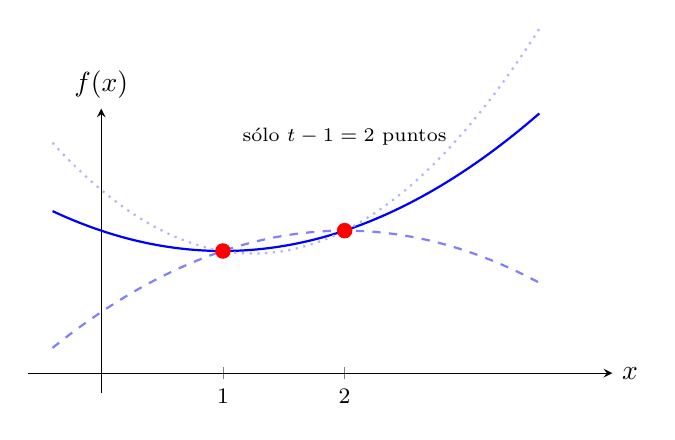
\begin{tikzpicture}
\begin{axis}[
  width=9cm, height=5.2cm,
  axis lines=middle,
  xlabel=$x$, ylabel=$f(x)$,
  xlabel style={right}, ylabel style={above},
  xmin=-0.6, xmax=4.2, ymin=-1, ymax=13,
  xtick={1,2}, ytick=\empty,
  xticklabel style={font=\footnotesize},
  samples=80, domain=-0.4:3.6, clip=false]
  % con t-1=2 puntos: infinitas parabolas pasan por ellos
  \addplot[thick, blue, smooth] {x^2 - 2*x + 7};
  \addplot[thick, blue!50, smooth, dashed] {-1*x^2 + 4*x + 3};
  \addplot[thick, blue!30, smooth, dotted] {2*x^2 - 5*x + 9};
  \addplot[only marks, mark=*, mark size=2.6pt, red] coordinates {(1,6) (2,7)};
  \node[font=\scriptsize, anchor=north] at (axis cs:2.0,12.5) {sólo $t-1=2$ puntos};
\end{axis}
\end{tikzpicture}
\end{center}
\diagcaption{Con \textbf{menos de $t$} sombras (aquí $t-1=2$ puntos) hay \textbf{infinitas} curvas de grado $t-1$ que pasan por ellas: el secreto $f(0)$ queda totalmente indeterminado (entropía máxima, seguridad perfecta tipo Shannon).}

\paragraph{Reparto (cifrado).} Sea $S$ el secreto, en $\mathbb{Z}_p$ con $p$ primo,
$p > n$ y $p > S$.
\begin{itemize}[leftmargin=1.4em]
  \item Tomar coeficientes aleatorios $a_1, \dots, a_{t-1} \in \{0,\dots,p-1\}$ y fijar
  $a_0 = S$.
  \item Armar el polinomio de grado $t-1$:
  \[
  f(x) = S + a_1 x + a_2 x^2 + \dots + a_{t-1} x^{t-1} \pmod{p}
  \]
  El término independiente $f(0) = S$ es el secreto.
  \item La \textbf{sombra} del participante $i$ es el par $(i,\, f(i) \bmod p)$, para
  $i = 1, \dots, n$.
\end{itemize}

\paragraph{Reconstrucción (descifrado) por interpolación de Lagrange en
$\mathbb{Z}_p$.} Con $t$ sombras cualesquiera $(x_j, y_j)$:
\[
S = f(0) = \sum_{j} y_j \, L_j(0) \pmod p,
\qquad
L_j(0) = \prod_{m \neq j} \frac{x_m}{x_m - x_j} \pmod p
\]
El \textbf{inverso modular} de $(x_m - x_j)$ se calcula con Euclides extendido o por
Fermat ($a^{-1} \equiv a^{p-2} \bmod p$).

\begin{ojo}
\textbf{Error típico:} fallar en la \textbf{aritmética modular} —no reducir mod $p$,
o invertir mal—. Cada división es una multiplicación por el inverso modular; no se
puede ``dividir'' directamente. Y en la parte (c) (ver abajo), no expresar el umbral
en términos de \textbf{entropía}.
\end{ojo}

\subsubsection{Ejemplo completo resuelto $(t,n)=(3,5)$ en $\mathbb{Z}_{11}$}

\textbf{Cifrado.} Secreto $S = 7$, esquema $(3,5)$ $\Rightarrow$ polinomio de grado
$t-1 = 2$:
\[
f(x) = 5x^2 + 3x + 7 \pmod{11}
\]
Sombras (evaluando en $x = 1,\dots,5$):
\begin{align*}
f(1) &= 5 + 3 + 7 = 15 \equiv 4 \pmod{11}\\
f(2) &= 20 + 6 + 7 = 33 \equiv 0 \pmod{11}\\
f(3) &= 45 + 9 + 7 = 61 \equiv 6 \pmod{11}\\
f(4) &= 80 + 12 + 7 = 99 \equiv 2 \pmod{11}\\
f(5) &= 125 + 15 + 7 = 147 \equiv 4 \pmod{11}
\end{align*}
Sombras: $(1,4),\ (2,0),\ (3,6),\ (4,2),\ (5,4)$.

\textbf{Descifrado} tomando tres cualesquiera, p.\ ej.\ $(2,0),(3,6),(5,4)$:
\begin{align*}
f(x) &= 0 \cdot \frac{(x-3)(x-5)}{(2-3)(2-5)} + 6 \cdot \frac{(x-2)(x-5)}{(3-2)(3-5)} + 4 \cdot \frac{(x-2)(x-3)}{(5-2)(5-3)}\\
&= \Big[\, 0 - 3(x^2 - 7x + 10) + \tfrac{4}{6}(x^2 - 5x + 6)\,\Big] \pmod{11}\\
&= 5x^2 + 3x + 7
\end{align*}
y el secreto es $\;s = f(0) = 7.\;$ \checkmark

\begin{examen}
\textbf{Ejemplo real adicional para practicar.} Esquema $(k,n)=(3,4)$ en
$\mathbb{Z}_7$, con $C=\{(1,6),(2,1),(3,0),(4,3)\}$. Recuperar el polinomio y el
secreto: el resultado esperado es
\[
f(x) = 1 + 3x + 2x^2 \pmod 7, \qquad S = f(0) = 1.
\]
Verificación rápida: $f(1)=1+3+2=6$; $f(2)=1+6+8=15\equiv 1$; $f(3)=1+9+18=28\equiv 0$;
$f(4)=1+12+32=45\equiv 3 \pmod 7$. \checkmark
\end{examen}

\begin{examen}
\textbf{Parte (c) típica: el umbral en términos de entropía.}
\begin{itemize}[leftmargin=1.3em]
  \item Con \textbf{menos de $t$ sombras}, la entropía del secreto $H(S)$ se mantiene
  \textbf{máxima}: no se filtra ninguna información (todos los valores del secreto
  siguen siendo igualmente probables) $\Rightarrow$ seguridad perfecta tipo Shannon.
  \item Con \textbf{$t$ sombras}, $H(S) = 0$: el secreto queda completamente
  determinado.
\end{itemize}
\end{examen}

\begin{destacado}
Shamir funciona sobre \textbf{cualquier cuerpo finito}, no solo $\mathbb{Z}_p$:
también sobre cuerpos de extensión $\mathbb{F}_{2^n}$.
\end{destacado}

\end{document}
